%%
%% Template intro.tex
%%

\chapter{An Introduction to My Thesis}
\label{cha:intro}
	Q\&A websites have been witnessing the 	unprecedented developemnt in the recent years. Although English is as close a global langauge, many Q\&A websites debates on the “English Only” language policy have never come to an end. According to the Wikipedia [2], English is the third place in the rank of first language speakers and second place for the first and the second language speakers. It means that there are nearly three-quarters of people in this world speak other languages. Some website like Quora insisted the English only policy, but the Spanish version of Quora was open on 19th Oct 2016. Another example is Stack Overflow, who has launched many other languages variants for users who are native speakers of other languages including Russian, Spanish and Japanese. \par
	\begin{table}[h!]
		\centering
		\caption{User amount and post amount of all Stack Overflow sites(By 1st Sep. 2017)}
		\label{tab:table1}
		\begin{tabular}{lrrr}
			Site & \#User & \#Post & \#Comment\\
			\hline
			Main site & 7,617,191  &  37,215,528 & 60,098,125\\
			Russian & 86,826 &  366,485 & 678,556\\
			Portuguese & 61,280 & 180,877& 322,241\\
			Spanish & 49,033 & 76,278 & 123,662\\
			Japanese & 13,457 & 28,589& 27,297\\
		\end{tabular}
	\end{table}
	
	Stack Overflow is a platform with millions of users and hundreds of millions of posts and answers. Table 1.1 presents the statistics of users, posts and comment of Stack Overflow main site and other language sites. As we can see, there exists a huge differences in user amount and post amount between the Stack Overflow main site and all other language variants. Therefore, it is meaningful if a clear answer can be found that whether Q\&A websites and communities should keep developing their multilingual variants, and more contributions can be made to bridging the lingual gap for all users who are not a native English speaker. It is highly believed that humans are accustomed to a more familiar environment [24], especially language environment. Although some people learn a second language, the native language is absolutely more attractive. However, the lingual gap between different language communities is hard to bridge. 

\par
	The active level of a community is determined by many factors, and the most important one is the amount of users, that is more people more interactions. Comparing the statistics in Tabel 1.1, it is clear that the number of user in Stack Overflow main site is 88 times that of Russian Stack Overflow, which means the gap of resources is enormous. There always exists a doubt that whether developers need to build multilingual communities. In this empirical study, our main research object is Russian Stack Overflow, which supports more users than other variants. Compared with the Stack Overflow main site, we will analyze how the activity of users from different language environment can influence communities and explore the importance of the multilingual Q\&A communities.\par
	
	\begin{figure}[!h]
	\centering
	\subfigure[Case 1 : No good solution on Russian Stack Overflow]{\label{fig:a}
		
\includegraphics[width = 0.80\textwidth]{figures/introex1.png}
	}
	\subfigure[Case 2 : Good solutions exist on Stack Overflow main site]{\label{fig:a}
		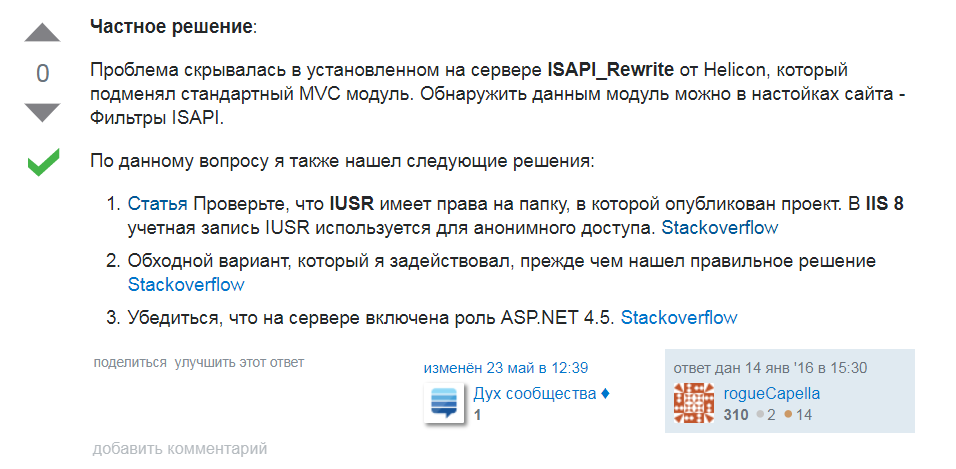
\includegraphics[width = 0.80\textwidth]{figures/introex2.png}
	}
	\caption{Examples of cross-lingual information needs}
	\label{fig}
\end{figure}
	There are several interesting cases on the sites of Stack Overflow, which are presented in Figure 1.1. The sub-figure a) shows a very common phenomenon that users from the other language subsite of Stack Overflow like the Russian variant often cannot find satisfying and high-quality answers on other language Stack Overflow sites, which need to be defined as {\bf sub-sites}, for some reasons, while the main site can alway assists them with the solutions. The sub-figure b) is a answer posted on Russian Stack Overflow, which means, in English, there are some previous solutions on the Stack Overflow English main site for this specific Russian question.  
\par
	Imagine that a Russian speaker who cannot speak English fail to find a good answer to his or her question. Meanwhile, the reply to his post is quite slow because the number of users on Russian Stackoverflow is small. For this problem, our cross-lingual deep learning model can efficiently deal with the lingual gap problem and recommend useful resources across different languages. A key benefit of this approach is the non-English speakers can efficiently utilize the huge knowledge base from the dominant English community.
	The main contributions of this paper are listed below:
	
	\begin{itemize}
		\item[*] A deep analysis of the value of multilingual communities and explore the user activity features in technical communities.
		\item[*] Mining duplicate post pairs that can be used for deep learning model for Stack Overflow duplicate question detection.
		\item[*] Build deep learning model for Stack Overflow duplicate question detection with high accuracy.
		\item[*] Build deep learning model for semantic similarity (DSSM) for comparing cross-lingual post similarity.
		\item[*] Qualitative analysis of our experimental results and the benefits of our approach.
	\end{itemize}
	\par

%%% Local Variables: 
%%% mode: latex
%%% TeX-master: "thesis"
%%% End: 
